\newpage
\section{Ôn tập chương 7}
\def\thoigian{90}%--Thời gian
\de{Đề số 1}{Chương VII. Bất phương trình bậc hai một ẩn}



\begin{center}
	\textbf{PHẦN 1 - CÂU TRẮC NGHIỆM NHIỀU PHƯƠNG ÁN LỰA CHỌN}
\end{center}
\Opensolutionfile{ans}[ans/ans-TN-0D7-Ontap-Deso1]
%Câu 1
\begin{ex}%[Dự án D - đợt 2 NH24-25 - Lê Hồ Quang Minh]%[0D7H1-2] 
	Cho tam thức $f(x)=ax^2+bx+c(a \neq 0)$, $\Delta=b^2-4ac$. Ta có $f(x) \leq 0$ với $\forall x \in \mathbb{R}$ khi và chỉ khi
	\choice
	{\True $\heva{&a<0 \\ &\Delta \leq 0}$}	
	{$\heva{&a \leq 0 \\ &\Delta<0}$}	
	{$\heva{&a<0 \\ &\Delta \geq 0}$}	
	{$\heva{&a>0 \\ &\Delta \leq 0}$}	
	\loigiai{
		Áp dụng định lý về dấu của tam thức bậc hai ta có $f(x) \leq 0$ với $\forall x \in \mathbb{R} \Leftrightarrow\heva{&a<0 \\ &\Delta \leq 0.}$
	}
\end{ex}
%Câu 2
\begin{ex}%[Dự án D - đợt 2 NH24-25 - Lê Hồ Quang Minh]%[0D7H1-2]
	Bảng xét dấu nào sau đây là bảng xét dấu của tam thức $f(x)=-x^{2}+6x-9$?
	\choice
	{
\begin{tikzpicture}
			\tkzTabInit[nocadre=true, lgt=1.2, espcl=2, deltacl=0.5]
			{$x$/0.7,$f(x)$/.7}
			{$-\infty$,$3$,$+\infty$}
			\tkzTabLine{,+,$0$,-,}
	\end{tikzpicture}}
	{
\begin{tikzpicture}
			\tkzTabInit[nocadre=true, lgt=1.2, espcl=2, deltacl=0.5]
			{$x$/0.7,$f(x)$/.7}
			{$-\infty$,$3$,$+\infty$}
			\tkzTabLine{,-,$0$,+,}
	\end{tikzpicture}}
	{
\begin{tikzpicture}
			\tkzTabInit[nocadre=true, lgt=1.2, espcl=2, deltacl=0.5]
			{$x$/0.7,$f(x)$/.7}
			{$-\infty$,$3$,$+\infty$}
			\tkzTabLine{,+,$0$,+,}
	\end{tikzpicture}}
	{\True 
\begin{tikzpicture}
			\tkzTabInit[nocadre=true, lgt=1.2, espcl=2, deltacl=0.5]
			{$x$/0.7,$f(x)$/.7}
			{$-\infty$,$3$,$+\infty$}
			\tkzTabLine{,-,$0$,-,}
	\end{tikzpicture}}
	\loigiai{
		Ta có $-x^{2}+6x-9=0\Leftrightarrow x=3$ và $a=-1<0$.
	}
\end{ex}
%Câu 3
\begin{ex}%[Dự án D - đợt 2 NH24-25 - Lê Hồ Quang Minh]%[0D7H1-2]
	Bảng xét dấu nào sau đây là bảng xét dấu của tam thức $f(x)=-x^{2}-x+6$?
	\choice
	{
\begin{tikzpicture}
			\tkzTabInit[nocadre=true, lgt=1.2, espcl=1.75, deltacl=0.5]
			{$x$/0.7,$f(x)$/.7}
			{$-\infty$,$-2$,$3$,$+\infty$}
			\tkzTabLine{,-,$0$,+,$0$,-,}
	\end{tikzpicture}}
	{
\begin{tikzpicture}
			\tkzTabInit[nocadre=true, lgt=1.2, espcl=1.75, deltacl=0.5]
			{$x$/0.7,$f(x)$/.7}
			{$-\infty$,$-2$,$3$,$+\infty$}
			\tkzTabLine{,+,$0$,-,$0$,+,}
	\end{tikzpicture}}
	{\True 
\begin{tikzpicture}
			\tkzTabInit[nocadre=true, lgt=1.2, espcl=1.75, deltacl=0.5]
			{$x$/0.7,$f(x)$/.7}
			{$-\infty$,$-3$,$2$,$+\infty$}
			\tkzTabLine{,-,$0$,+,$0$,-,}
	\end{tikzpicture}}
	{
\begin{tikzpicture}
			\tkzTabInit[nocadre=true, lgt=1.2, espcl=1.75, deltacl=0.5]
			{$x$/0.7,$f(x)$/.7}
			{$-\infty$,$-3$,$2$,$+\infty$}
			\tkzTabLine{,+,$0$,-,$0$,+,}
	\end{tikzpicture}}
	\loigiai{
		Ta có $-x^{2}-x+6=0\Leftrightarrow\hoac{&x=2\\&x=-3}$ và $a=-1<0$.
	}
\end{ex}
%Câu 4
\begin{ex}%[Dự án D - đợt 2 NH24-25 - Lê Hồ Quang Minh]%[0D7H1-2]
	Cho tam thức bậc hai $f(x)=x^{2}+1$. Mệnh đề nào sau đây đúng?
	\choice
	{\True $f(x)>0\Leftrightarrow x\in(-\infty;+\infty)$}
	{$f(x)=0\Leftrightarrow x=-1$}
	{$f(x)<0\Leftrightarrow x\in(-\infty;1)$}
	{$f(x)>0\Leftrightarrow x\in(0;1)$}
	\loigiai{
		Ta có $f(x)=x^{2}+1\geq 1>0$, $\forall x\in \mathbb{R}$.
	}
\end{ex}
%Câu 5
\begin{ex}%[0D7N2-1]%[Dự án D - đợt 2 NH24-25 - Lê Hồ Quang Minh]
	Tập nghiệm của bất phương trình $x^2-25<0$ là
	\choice
	{\True $S=(-5;5)$}
	{$ x>\pm 5$}
	{$-5<x<5$}
	{$S=(-\infty ;-5)\cup (5;+\infty)$}
	\loigiai{
		Bất phương trình $x^2-25<0$$\Leftrightarrow -5<x<5$.\\
		Vậy $S=(-5;5)$.
	}
\end{ex}
%Câu 6
\begin{ex}%[0D7N2-1]%[Dự án D - đợt 2 NH24-25 - Lê Hồ Quang Minh]
	Tập xác định của hàm số $y=\sqrt{-x^2+2x+3}$ là
	\choice
	{$(1;3)$}
	{$(-\infty ;-1)\cup (3;+\infty)$}
	{\True $[-1;3]$}
	{$(-\infty ;-1]\cup [3;+\infty)$}
	\loigiai{
		Hàm số $y=\sqrt{-x^2+2x+3}$ xác định khi $-x^2+2x+3\ge 0\Leftrightarrow -1\le x\le 3$.\\
		Vậy tập xác định của hàm số là $D=[-1;3]$.
	}
\end{ex}
%Câu 7
\begin{ex}%[0D7H3-2]%%[Dự án D - đợt 2 NH24-25 - Lê Hồ Quang Minh]
	Tập nghiệm của phương trình $\sqrt{2x-1}=2-x$ là
	\choice
	{$S=\{ 1;5 \} $}
	{\True $S=\{ 1 \} $}
	{$S=\{ 5 \} $}
	{$S=\{ 2;3 \} $}
	\loigiai{
		Thay các giá trị vào phương trình có $ x=1$ vào thỏa mãn phương trình.
	}
\end{ex}

%Câu 8
\begin{ex}%[0D7N3-2]%[Dự án D - đợt 2 NH24-25 - Lê Hồ Quang Minh]
	Tập nghiệm của phương trình $\sqrt{2x-1}=-x^2-5$ là
	\choice
	{$S=\{ 1;5 \} $}
	{$S=\{ 1 \} $}
	{$S=\{ 5 \} $}
	{\True $S=\varnothing $}
	\loigiai{
		Vì $-x^2-5<0$ vậy phương trình vô nghiệm.
	}
\end{ex}
%Câu 9
\begin{ex}%[0D7H3-2]%[Dự án D - đợt 2 NH24-25 - Lê Hồ Quang Minh]
	Tìm số giao điểm giữa đồ thị hàm số $y=\sqrt{3x-4}$ và đường thẳng $y=x-3$.
	\choice
	{$2$ giao điểm}
	{$4$ giao điểm}
	{$3$ giao điểm}
	{\True $1$ giao điểm}
	\loigiai{
		Xét phương trình hoành độ giao điểm $\sqrt{3x-4}=x-3. \quad (1)$\\
		Ta có $(1) \Leftrightarrow \heva{& x-3\ge 0\\& 3x-4=x^2-6x+9} \Leftrightarrow \heva{&x\ge 3\\&x^2-9x+13=0} \Leftrightarrow \heva{&x\ge 3\\& x=\dfrac{9\pm\sqrt{29}}{2}} \Leftrightarrow x=\dfrac{9+\sqrt{29}}{2}.$\\
		Vậy đồ thị hàm số $y=\sqrt{3x-4}$ và đường thẳng $y=x-3$ có $1$ giao điểm chung.
	}
\end{ex}

%Câu 10

\begin{ex}%[0D7H2-6]%[Dự án D - đợt 2 NH24-25 - Lê Hồ Quang Minh]
	Tìm $m$ để phương trình $-x^2+2(m-1)x+m-3=0$ có hai nghiệm phân biệt
	\choice
	{$(-1;2)$}
	{\True $(-\infty ;-1)\cup (2;+\infty)$}
	{$[-1;2]$}
	{$(-\infty ;-1]\cup [2;+\infty)$}
	\loigiai{
		Phương trình có hai nghiệm phân biệt khi
		$$\Delta'>0\Leftrightarrow (m-1)^2-(-1)\cdot (m-3)>0\Leftrightarrow m^2-m-2>0\Leftrightarrow \hoac{& m<-1\\& m>2.}$$
		Vậy $ m\in (-\infty ;-1)\cup (2;+\infty)$.
	}
\end{ex}

%Câu 11
\begin{ex}%[0D7H2-6]%[Dự án D - đợt 2 NH24-25 - Lê Hồ Quang Minh]
	Tam thức $f(x)=x^2+2(m-1)x+m^2-3m+4$ không âm với mọi giá trị của $x$ khi
	\choice
	{$m<3$}
	{$m\ge 3$}
	{$m\le -3$}
	{\True $m\le 3$}
	\loigiai{
		Yêu cầu bài toán $\Leftrightarrow f(x)\ge 0,\forall x\in \mathbb{R} \Leftrightarrow\Delta'={{(m-1)}^2}-(m^2-3m+4)\le 0 \Leftrightarrow m-3\le 0 \Leftrightarrow m\le 3.$\\
		Vậy $m\le 3$ thỏa mãn yêu cầu bài toán.}
\end{ex}
%Câu 12
\begin{ex}%[0D7V2-6]%[Dự án D - đợt 2 NH24-25 - Lê Hồ Quang Minh]
	Tìm tất cả các giá trị của tham số $m$ để bất phương trình $\dfrac{-x^2+2x-5}{x^2-mx+1}\le 0$ nghiệm đúng với mọi $x\in \mathbb{R}$.
	\choice
	{$m\in \varnothing $}
	{$m\in (-2;2)$}
	{$m\in (-\infty ;-2]\cup[2;+\infty)$}
	{\True $m\in[-2;2]$}
	\loigiai{
		Ta có $-x^2+2x-5=-(x-1)^2-4<0,\forall x\in \mathbb{R}$.\\
		Nên $\dfrac{-x^2+2x-5}{x^2-mx+1}\le 0,\forall x\in \mathbb{R}$ khi $x^2-mx+1>0,\forall x\in \mathbb{R} \Leftrightarrow\Delta =m^2-4\le 0 \Leftrightarrow -2 \le m \le 2.$\\
		Vậy $m\in[-2;2]$.
	}
\end{ex}

\Closesolutionfile{ans}
%\begin{center}
%	\textbf{ĐÁP ÁN}
%	\inputansbox{10}{ans/ans}	
%\end{center}

\begin{center}
	\textbf{PHẦN 2 - CÂU TRẮC NGHIỆM ĐÚNG SAI}
\end{center}
\setcounter{ex}{0}
\Opensolutionfile{ans}[ans/ans-DS-0D7-Ontap-Deso1]
%Câu 1
\begin{ex}%[Dự án D - đợt 2 NH24-25 - Lê Hồ Quang Minh]%[0D7H1-3]	
	Cho đồ thị hàm số bậc hai $y=f(x)$ và $y=g(x)$.
	\begin{center}
		\begin{tikzpicture}[scale=0.8, font=\footnotesize, line join=round,
			line cap=round, >=stealth]
			\begin{scope}[xshift=0cm,yshift=0,line join=round, line cap=round,scale=1,transform shape]
				\def \xmin{-3}
				\def \xmax{3}
				\def \ymin{-4.5}
				\def \ymax{1}
				\draw[->] (\xmin,0)--(\xmax,0) node[shift=(-110:0.2)] {$x$};
				\draw[->] (0,\ymin)--(0,\ymax) node[shift=(-150:0.2)] {$y$};
				\fill (0,0) circle(1pt) node[shift=(-45:0.25)]{$O$}
				(-2,0) circle(1pt) node[shift=(-135:0.3)]{$-2$}
				(2,0) circle(1pt) node[shift=(-45:0.3)]{$2$}
				(0,-4) circle(1pt) node[shift=(-150:0.3)]{$-4$};
				\clip (\xmin,\ymin) rectangle (\xmax,\ymax);
				\draw[smooth,samples=100,domain=\xmin:\xmax] plot(\x,{(\x)^2-4});
				
			\end{scope}
			\begin{scope}[xshift=5cm,yshift=0,line join=round, line cap=round,scale=1,transform shape]
				\def \xmin{-1}
				\def \xmax{7}
				\def \ymin{-4}
				\def \ymax{1.5}
				\draw[->] (\xmin,0)--(\xmax,0) node[shift=(-110:0.2)] {$x$};
				\draw[->] (0,\ymin)--(0,\ymax) node[shift=(-150:0.2)] {$y$};
				\fill (0,0) circle(1pt) node[shift=(-135:0.25)]{$O$}
				(3,0) circle(1pt) node[shift=(135:0.3)]{$3$}
				(4,0) circle(1pt) node[shift=(45:0.3)]{$4$}
				(0,1) circle(1pt) node[shift=(180:0.3)]{$1$};
				\clip (\xmin,\ymin) rectangle (\xmax,\ymax);
				\draw[smooth,samples=100,domain=\xmin:\xmax] plot(\x,{-(\x)^2+7*(\x)-12});
			\end{scope}
			\fill (0,-5) node {$y=f(x)$};
			\fill (8,-5) node {$y=g(x)$};
		\end{tikzpicture}
	\end{center}
	\choiceTF
	{\True Đồ thị hàm số $y=f(x)$ cắt trục hoành tại hai điểm $(-2;0)$ và $(2;0)$}
	{\True Đồ thị hàm số $y=g(x)$ cắt trục hoành tại hai điểm $(3;0)$ và $(4;0)$}
	{Tam thức bậc hai $f(x)$ có bảng xét dấu\\
			
\begin{tikzpicture}
				\tkzTabInit[nocadre=true, lgt=1.2, espcl=2, deltacl=0.5]
				{$x$/0.7,$f(x)$/.7}
				{$-\infty$,$-2$,$2$,$+\infty$}
				\tkzTabLine{,-,$0$,+,$0$,-,}
			\end{tikzpicture}
	}
	{\True $g(x)>0\Leftrightarrow 3<x<4$}
	\loigiai{
		\begin{itemchoice}
			\itemch Quan sát đồ thị hàm số $y=f(x)$, ta thấy đồ thị hàm số $y=f(x)$ cắt trục hoành tại hai điểm $(-2;0)$ và $(2;0)$.
			\itemch Quan sát đồ thị hàm số $y=g(x)$, ta thấy đồ thị hàm số $y=g(x)$ cắt trục hoành tại hai điểm $(3;0)$ và $(4;0)$.		
			\itemch Ta có bảng xét dấu
			\begin{center}
				
\begin{tikzpicture}
					\tkzTabInit[nocadre=true, lgt=1.2, espcl=2, deltacl=0.5]
					{$x$/0.7,$f(x)$/.7}
					{$-\infty$,$-2$,$2$,$+\infty$}
					\tkzTabLine{,+,$0$,-,$0$,+,}
				\end{tikzpicture}
			\end{center}
			\itemch Quan sát đồ thị hàm số $y=g(x)$, ta thấy $g(x)>0\Leftrightarrow 3<x<4$.
		\end{itemchoice}
	}
\end{ex}

%Câu 2
\begin{ex}%[0D7V3-1]%[Dự án D - đợt 2 NH24-25 - Lê Hồ Quang Minh]
	Cho phương trình $(x-2)\sqrt{2x^2+4}=x^2-4$. Khi đó
	\choiceTF
	{Điều kiện $x\geq2$}
	{\True Phương trình có $3$ nghiệm}
	{Tổng các nghiệm của phương trình bằng $5$}
	{\True Các nghiệm của phương trình đều là các số chẵn}
	\loigiai{
		\begin{itemchoice}
			\itemch Điều kiện $2x^2+4\geq0 , \forall x \in \mathbb{R}$.
			\itemch Ta có
			$(x-2)\sqrt{2x^2+4}=x^2-4\Leftrightarrow (x-2)\sqrt{2x^2+4}=(x-2)(x+2)\Leftrightarrow \hoac{& x-2=0 \\ & \sqrt{2x^2+4}=x+2}$\\
			$\Leftrightarrow \hoac{& x=2 \\ & \heva{& x+2 \geq 0 \\ & 2x^2+4=x^2+4x+4}}\Leftrightarrow \hoac{& x=2 \\ & \heva{& x \geq -2 \\ & x^2-4x=0}} \Leftrightarrow \hoac{& x=2 \\ & \heva{& x \geq -2 \\ & x=0 \lor x=4}} \Leftrightarrow \hoac{& x=2 \\ & x=0 \\ & x=4.}$\\
			Vậy tập nghiệm của phương trình là $S=\{0;2;4\}$.
			\itemch Tổng các nghiệm của phương trình bằng $6$.
			\itemch Các nghiệm của phương trình là các số chẵn.
		\end{itemchoice}
	}
\end{ex}

\Closesolutionfile{ans}
%\inputansbox[2]{2}{ans/answer.tex}



\begin{center}
	\textbf{PHẦN 3 - CÂU TRẮC NGHIỆM TRẢ LỜI NGẮN}
\end{center}
\setcounter{ex}{0}
\Opensolutionfile{ans}[ans-KQ-0D7-Ontap-Deso1]

% Câu 1
 \begin{ex}%[0D7H3-4]%[Dự án D - đợt 2 NH24-25 - Lê Hồ Quang Minh]
 	Tính tổng các phần tử trong tập nghiệm của phương trình $\sqrt{3x^2-9x+1}=|x-2|$.
 	\shortans[oly]{$0{,}5$}
 	\loigiai{
 		Bình phương hai vế phương trình, ta có
 			$ 3x^2-9x-5=x^2-8x+16\Leftrightarrow 2x^2-x-21=0\Leftrightarrow \hoac{&x=-3\\ &x=\dfrac{7}{2}.}$
 			\begin{itemize}
 				\item Thay $x=-3$ vào phương trình, ta được $\sqrt{49}=|-7|$ (thỏa mãn).
 				\item Thay $x=\dfrac{7}{2}$ vào phương trình, ta được $\dfrac{1}{2}=\left|-\dfrac{1}{2}\right|$ (thỏa mãn).
 			\end{itemize}			
 			Vậy tập nghiệm phương trình là $S=\left\{-3; \dfrac{7}{2}\right\}$.\\
 		Vậy tổng các phần tử trong tập nghiệm của phương trình là $-3+\dfrac{7}{2}=\dfrac{1}{2}$.
 	}
 \end{ex}
\begin{ex}%[0D7V2-6]
	Có bao nhiêu giá trị nguyên của tham số $m$, hàm số $y=\sqrt{x^2-2mx+m-1}$ có tập xác định là $\mathbb{R}$?
	\shortans{$0$}
	\loigiai{
		Để hàm số $y=\sqrt{x^2-2mx+m-1}$ có tập xác định là $\mathbb{R}$ thì \[x^2-2mx+m-1\ge 0,\,\forall x\in \mathbb{R}\Leftrightarrow\heva{&{a > 0} \\
			&{\Delta \le 0}&}\Leftrightarrow\heva{&1>0\\&m^2-m+1\leq 0\;(*)}.\]
		Vì $\left(m-\dfrac{1}{2}\right)^2+\dfrac{3}{4}>0,\,\forall x$ nên (*) vô nghiệm.\\
		Vậy không tồn tại giá trị của tham số $m$ để thoả mãn yêu cầu bài toán.
	}
\end{ex}
% Câu 2
\begin{ex}%[0D7V3-6]%[Dự án D - đợt 2 NH24-25 - Lê Hồ Quang Minh]
	\immini{
		Cho nửa đường tròn đường kính $MN=10$. Cho điểm $B$ (không trùng hai điểm $M$, $N$) di động trên nửa đường tròn và hình chiếu của $B$ trên đoạn $MN$ là điểm $A$, vẽ hình chữ nhật $ABCD$ với $C$ cũng thuộc nửa đường tròn. Tìm độ dài $IA$ biết rằng chu vi hình chữ nhật $ABCD$ bằng $22$ và độ dài $IA$ là một số nguyên.
	}{
		\begin{tikzpicture}[>=stealth,line join=round,line cap=round,font=\footnotesize,scale=1]
			\def\r{3};
			\def\g{130};
			\path
			(0,0) coordinate (I)
			(0:\r) coordinate (N)
			(180:\r) coordinate (M)
			(\g:\r) coordinate (B)
			(180-\g:\r) coordinate (C)
			($(M)!(B)!(N)$) coordinate (A)
			($(M)!(C)!(N)$) coordinate (D)
			;
			\pgfresetboundingbox
			\draw (N) arc(0:180:\r)--cycle
			(A)--(B)--(C)--(D) (I)--(B)
			;
			\foreach \x/\g in {A/-90,I/-90,B/130,C/50,D/-90,N/0}\fill[black](\x) circle (1pt) +(\g:3mm) node {$\x$};
			\foreach \x/\y/\z in {A/B/C,B/C/D,C/D/A,B/A/D}{\draw pic[draw,angle radius=2mm]{right angle=\x--\y--\z};}
		\end{tikzpicture}
	}
	\shortans[oly]{$4$}
	\loigiai{
		Đặt $IA=x \in(0; 5) \Rightarrow AD=2x$.\\
		Xét tam giác $IAB$ vuông tại $A$, ta có $AB=\sqrt{5^2-x^2}$.\\
		Theo đề bài, ta có phương trình
		\begin{eqnarray*}
			& & 2AB+2AD=22\\
			& \Leftrightarrow & 4x+2\sqrt{5^2-x^2}=22\\
			& \Leftrightarrow & \sqrt{25-x^2}=11-2x\\
			& \Leftrightarrow & \heva{&11-2x \geq 0\\ &25-x^2=121-44x+4x^2}\\
			& \Leftrightarrow & \heva{&x \leq \dfrac{11}{2} \\ &5x^2-44x+96=0}\\
			& \Leftrightarrow & \heva{&x \leq \dfrac{11}{2} \\ &\hoac{&x=4\\&x=\dfrac{24}{5}}}\\
			& \Leftrightarrow & \hoac{&x=4\\&x=\dfrac{24}{5}.}
		\end{eqnarray*}
		Vậy $IA=4$.
	}
\end{ex}

%Câu 3
\begin{ex}%[0D7V3-6]%[Dự án D - đợt 2 NH24-25 - Lê Hồ Quang Minh]
	Lúc $8$ giờ sáng, hai ô tô cùng xuất phát tại vị trí $A$ và vị trí $B$ cách nhau $100$ km chạy về thành phố $T$. Vận tốc của hai ô tô chạy từ vị trí $A$ và vị trí $B$ lần lượt là $55$ km/h và $45$ km/h. Biết rằng tại thời điểm ô tô đi từ vị trí $A$ đến địa điểm $D$ cách thành phố $T$ $14$ km thì ô tô đi từ vị trí $B$ đến địa điểm $C$ cách thành phố $T$ là $6$ km. Thời điểm đó là $a$ giờ $b$ phút. Tính $a+b$.
	\begin{center}
		\tikzset{every picture/.style={line width=0.75pt}} %set default line width to 0.75pt
		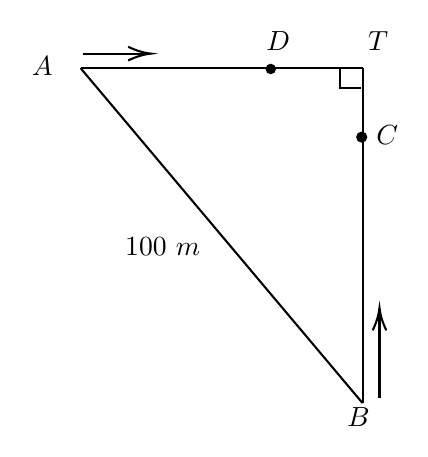
\begin{tikzpicture}[x=0.75pt,y=0.75pt,yscale=-1,xscale=1]
			\draw    (310,99) -- (445.87,260.4) ;
			\draw    (445.87,99) -- (445.87,260.4) ;
			\draw    (310,99) -- (445.87,99) ;
			\draw    (311,92) -- (341.87,92) ;
			\draw [shift={(343.87,92)}, rotate = 180] [color={rgb, 255:red, 0; green, 0; blue, 0 }  ][line width=0.75]    (10.93,-3.29) .. controls (6.95,-1.4) and (3.31,-0.3) .. (0,0) .. controls (3.31,0.3) and (6.95,1.4) .. (10.93,3.29)   ;
			\draw    (454,258) -- (454,216.4) ;
			\draw [shift={(454,214.4)}, rotate = 90] [color={rgb, 255:red, 0; green, 0; blue, 0 }  ][line width=0.75]    (10.93,-3.29) .. controls (6.95,-1.4) and (3.31,-0.3) .. (0,0) .. controls (3.31,0.3) and (6.95,1.4) .. (10.93,3.29)   ;
			\draw   (445,108.4) -- (434.87,108.4) -- (434.87,99) ;
			\draw  [color={rgb, 255:red, 0; green, 0; blue, 0 }  ,draw opacity=1 ][fill={rgb, 255:red, 0; green, 0; blue, 0 }  ,fill opacity=1 ] (399.6,99.4) .. controls (399.6,98.3) and (400.5,97.4) .. (401.6,97.4) .. controls (402.7,97.4) and (403.6,98.3) .. (403.6,99.4) .. controls (403.6,100.5) and (402.7,101.4) .. (401.6,101.4) .. controls (400.5,101.4) and (399.6,100.5) .. (399.6,99.4) -- cycle ;
			\draw  [color={rgb, 255:red, 0; green, 0; blue, 0 }  ,draw opacity=1 ][fill={rgb, 255:red, 0; green, 0; blue, 0 }  ,fill opacity=1 ] (443.27,132.23) .. controls (443.27,131.04) and (444.24,130.07) .. (445.43,130.07) .. controls (446.63,130.07) and (447.6,131.04) .. (447.6,132.23) .. controls (447.6,133.43) and (446.63,134.4) .. (445.43,134.4) .. controls (444.24,134.4) and (443.27,133.43) .. (443.27,132.23) -- cycle ;
			\draw (447,80) node [anchor=north west][inner sep=0.75pt]   [align=left] {$\displaystyle T$};
			\draw (330,179) node [anchor=north west][inner sep=0.75pt]   [align=left] {$\displaystyle 100\ \text{m}$};
			\draw (285,92) node [anchor=north west][inner sep=0.75pt]   [align=left] {$\displaystyle A$};
			\draw (437,261) node [anchor=north west][inner sep=0.75pt]   [align=left] {$\displaystyle B$};
			\draw (451,125) node [anchor=north west][inner sep=0.75pt]   [align=left] {$\displaystyle C$};
			\draw (398,80) node [anchor=north west][inner sep=0.75pt]   [align=left] {$\displaystyle D$};
		\end{tikzpicture}
	\end{center}
	\shortans[oly]{$21$}
	\loigiai{
		Gọi $x$ (giờ) là thời gian ô tô đi từ vị trí $A$ đến địa điểm $D\ (x>0)$.\\
		Vì hai ô tô xuất phát cùng một lúc nên thời gian ô tô đi từ vị trí $B$ đến địa điểm $C$ cũng là $x$ giờ.\\
		Do đó, quãng đường $AD$ và $BC$ lần lượt là $55x$ km và $45x$ km.\\
		Suy ra khoảng cách từ vị trí $A$ và vị trí $B$ đến thành phố $T$ lần lượt là $55x+14$ km và $45x+6$ km.\\
		Vì khoảng cách giữa hai vị trí $A$ và $B$ là $100$ km nên ta có phương trình
		$$\sqrt{(55x+14)^2+(45x+6)^2}=100\Rightarrow 5\,050x^2+2\,080x+232=10\,000.$$
		Giải phương trình này và kết hợp với điều kiện $x>0$, ta nhận $x=\dfrac{6}{5}$.\\
		Đổi $\dfrac{6}{5}$ giờ $=1$ giờ $12$ phút.\\
		Vậy thời điểm ô tô đi từ vị trí $A$ đến địa điểm $D$ là
		8 giờ $+1$ giờ $12$ phút $=9$ giờ $12$ phút (sáng).\\
		Khi đó $\heva{& a=9 \\ & b=12} \Rightarrow a+b=21$.
	}
\end{ex}
\Closesolutionfile{ans}

\begin{center}
	\textbf{PHẦN 4 - TỰ LUẬN}
\end{center}
\setcounter{ex}{0}
% Câu 1
\begin{ex}%[0D7H2-6]%[Dự án D - đợt 2 NH24-25 - Lê Hồ Quang Minh]
	Tìm tất cả các giá trị của tham số $m$ để phương trình $-x^{2} +x+4m^{2} -5m+1=0$ có hai nghiệm trái dấu.		

	\loigiai{
		Để phương trình $-x^{2} +x+4m^{2} -5m+1=0$ có hai nghiệm trái dấu thì $x_{1} \cdot x_{2} <0\Leftrightarrow -4m^{2} +5m-1<0.$\\
		Giải bất phương trình trên ta được $m<\dfrac{1}{4} $ hoặc $m>1$.\\
		Vậy để phương trình có hai nghiệm trái dấu thì $m\in \left(-\infty ;\dfrac{1}{4} \right)\cup (1;+\infty )$.
	}
\end{ex}
% Câu 2
\begin{ex}%[0D7H2-7]%[Dự án D - đợt 2 NH24-25 - Lê Hồ Quang Minh]
	Bộ phận nghiên cứu thị trường của một xí nghiệp xác định tổng chi phí để sản xuất $Q$ sản phẩm là $Q^{2} +300Q+200\,000$ (nghìn đồng). Giả sử giá mỗi sản phẩm bán ra thị trường là $1\,200$ nghìn đồng. Hãy xác định số sản phẩm tối thiểu và tối đa mà xí nghiệp cần sản xuất để không bị lỗ.
	\loigiai{
		Lợi nhuận của xí nghiệp khi bán hết $Q$ sản phẩm là 
		\[1\,200Q-\left(Q^{2} +300Q+200\,000\right)=-Q^{2} +900Q-200\,000.\] 
		Để xí nghiệp không bị lỗ thì $-Q^{2} +900Q-200\,000\ge 0\Leftrightarrow 400\le Q\le 500$.\\
		Vậy để không bị lỗ, xí nghiệp cần sản xuất tối thiểu $400$ sản phẩm và tối đa $500$ sản phẩm.
	}
\end{ex}
% Câu 3
\begin{ex}%[0D7V3-6]%[Dự án D - đợt 2 NH24-25 - Lê Hồ Quang Minh]
	Một chú thỏ ngày nào cũng ra bờ suối ở vị trí $A$, cách cửa hang của mình tại vị trí $B$ là $370$ m để uống nước, sau đó chú thỏ sẽ đến vị trí $C$ cách vị trí $A$ $120$ m để ăn cỏ rồi trở về hang. Tuy nhiên, hôm nay sau khi uống nước ở bờ suối, chú thỏ không đến vị trí $C$ như mọi ngày mà chạy đến vị trí $D$ (thuộc $BC$) để tìm cà rốt rồi mới trở về hang (xem hình bên dưới). Biết rằng, tổng thời gian chú thỏ chạy từ vị trí $A$ đến vị trí $D$ rồi về hang là $30$ giây (không kể thời gian tìm cà rốt), trên đoạn $AD$ chú thỏ chạy với vận tốc là $13\ \mathrm{m/s}$, trên đoạn $BD$ chú thỏ chạy với vận tốc là $15\ \mathrm{m/2}$. Vị trí $C$ cách vị trí $D$ bao nhiêu mét?
	\begin{center}
		\begin{tikzpicture}[>=stealth,line join=round,line cap=round,font=\footnotesize,scale=1]
			\def\a{12};
			\def\b{35};
			\path
			(0,0) coordinate (C)
			(0:0.25*\b) coordinate (B)
			(-90:0.25*\a) coordinate (A)
			($(C)!1/7!(B)$) coordinate (D)
			;
			\pgfresetboundingbox
			\draw
			(C)--(A)node[midway,sloped,above]{\scriptsize $120$ m}--(B)node[midway,sloped,above]{\scriptsize $370$ m}--cycle (A)--(D)
			;
			\foreach \x/\g in {B/0,C/-135,A/-90,D/90}\fill[black](\x) circle (1pt) +(\g:3mm) node {$\x$};
		\end{tikzpicture}
	\end{center}
	\loigiai{
		Gọi thời gian chú thỏ chạy trên đoạn $AD$ là $x\ (0< x < 30)$ (giây),\\
		Khi đó thời gian chú thỏ chạy trên đoạn $BD$ là $30-x$ (giây).\\
		Do đó, quãng đường $AD$ và $BD$ lần lượt là $13x$ (m) và $15(30-x)$ (m).\\
		Độ dài quãng đường $BC$ là $\sqrt{370^2-120^2}=350\ (\mathrm{m})$.\\
		Tam giác $ACD$ vuông tại $C$ nên
		$CD=\sqrt{(13x)^2-120^2}=\sqrt{169x^2-14400}\ (\mathrm{m}).$\\
		Mặt khác, $CD=BC-BD=350-15(30-x)$ (m).\\
		Do đó, ta có phương trình
		$\sqrt{169x^2-14\,400}=350-15(30-x)\Leftrightarrow 56x^2-3\,000x+24\,400=0.$\\
		Giải phương trình này và kết hợp với điều kiện $0< x < 30$, ta nhận $x=10$ giây.\\
		Vậy khoảng cách giữa vị trí $C$ và vị trí $D$ là $350-15(30-10)=50$ m.
	}
\end{ex}
